% Intended LaTeX compiler: pdflatex
\documentclass[11pt]{article}
\usepackage[utf8]{inputenc}
\usepackage[T1]{fontenc}
\usepackage{graphicx}
\usepackage{longtable}
\usepackage{wrapfig}
\usepackage{rotating}
\usepackage[normalem]{ulem}
\usepackage{amsmath}
\usepackage{amssymb}
\usepackage{capt-of}
\usepackage{hyperref}
\author{Construção de compiladores I}
\date{}
\title{Análise sintática}
\hypersetup{
 pdfauthor={Construção de compiladores I},
 pdftitle={Análise sintática},
 pdfkeywords={},
 pdfsubject={},
 pdfcreator={Emacs 28.2 (Org mode 9.7)}, 
 pdflang={English}}
\begin{document}

\maketitle
\section*{Objetivos}
\label{sec:org066f1a2}

\subsection*{Objetivos}
\label{sec:orgdc9e617}

\begin{itemize}
\item Introduzir a segunda etapa do front-end: a análise sintática.

\item Introduzir o conceito de analisadores top-down e bottom-up.
\end{itemize}
\subsection*{Objetivos}
\label{sec:org78c66fb}

\begin{itemize}
\item Apresentar a técnica de análise sintática descendente recursiva.
\end{itemize}
\section*{Análise sintática}
\label{sec:org8d4c109}

\subsection*{Análise sintática}
\label{sec:org4225fdc}

\begin{itemize}
\item Responsável por determinar se o programa atende as restrições sintáticas
da linguagem.
\end{itemize}
\subsection*{Análise sintática}
\label{sec:orgdceca08}

\begin{itemize}
\item Regras sintáticas de uma linguagem são expressas utilizando gramáticas livres de contexto.
\end{itemize}
\subsection*{Análise sintática}
\label{sec:orgfbfa558}

\begin{itemize}
\item Porque utilizar GLCs e não ERs?
\begin{itemize}
\item ERs não são capazes de representar construções simples de linguagens.
\end{itemize}
\end{itemize}
\subsection*{Análise sintática}
\label{sec:orgeb66abe}

\begin{itemize}
\item Vamos considerar um fragmento de expressões formado por variáveis, constantes inteiras
adição, multiplicação.
\end{itemize}
\subsection*{Análise sintática}
\label{sec:orgc7c9d49}

\begin{itemize}
\item A seguinte ER representa essa linguagem:
\end{itemize}

\begin{array}{c}
base = [a..z]([a..z] | [0..9])^* \\
base((+|*)base)^*
\end{array}
\subsection*{Análise sintática}
\label{sec:orga5db16e}

\begin{itemize}
\item A ER anterior aceita palavras como \(a * b + c\).

\item Porém, como determinar a precedência entre operadores?
\end{itemize}
\subsection*{Análise sintática}
\label{sec:org603c844}

\begin{itemize}
\item Podemos usar a precedência usual da aritmética.

\item Porém, não é possível impor uma ordem diferente de avaliação.
\begin{itemize}
\item Para isso, precisamos de parêntesis.
\end{itemize}
\end{itemize}
\subsection*{Análise sintática}
\label{sec:org95272e4}

\begin{itemize}
\item Ao incluir parêntesis, temos um problema:
\begin{itemize}
\item Como expressar usando ER que parêntesis estão corretos?
\end{itemize}
\end{itemize}
\subsection*{Análise sintática}
\label{sec:orgbe2b490}

\begin{itemize}
\item Pode-se provar que a linguagem de parêntesis balanceados não é regular.
\begin{itemize}
\item Usando o lema do bombeamento.
\item Estrutura similar a \(\{0^n1^n\,|\,n\geq 0\}\).
\end{itemize}
\end{itemize}
\subsection*{Análise sintática}
\label{sec:orgfb76efd}

\begin{itemize}
\item Dessa forma, precisamos utilizar GLCs para representar a estrutura sintática
de linguagens.
\end{itemize}
\subsection*{Análise sintática}
\label{sec:org97dd7e3}

\begin{itemize}
\item Antes de apresentar técnicas de análise sintática, vamos revisar alguns
conceitos sobre GLCs.
\end{itemize}
\section*{Gramáticas Livres de Contexto}
\label{sec:org6c84d6f}

\subsection*{Gramáticas livres de contexto}
\label{sec:org00a69b1}

\begin{itemize}
\item Uma GLC é \(G=(V,\Sigma,R,P)\), em que
\begin{itemize}
\item \(V\): conjunto de variáveis (não terminais)
\item \(\Sigma\): alfabeto (terminais)
\item \(R \subseteq V\times (V\cup\Sigma)^*\): regras (produções).
\item \(P\in V\): variável de partida.
\end{itemize}
\end{itemize}
\subsection*{Gramáticas livres de contexto}
\label{sec:org1bc5414}

\begin{itemize}
\item Gramática de expressões
\end{itemize}

\begin{array}{lcl}
E & \to & (E) \,|\, E + E \,|\, E * E\,|\, num\,|\,var\\
\end{array}
\subsection*{Gramáticas livres de contexto}
\label{sec:org998dde8}

\begin{itemize}
\item \(V = \{E\}\)
\item \(\Sigma = \{num, var, (, ), *, +\}\)
\item \(R\): conjunto de regras da gramática.
\end{itemize}
\subsection*{Gramáticas livres de contexto}
\label{sec:orge7d786d}

\begin{itemize}
\item Determinamos se uma palavra pertence ou não à linguagem
de uma gramática construindo uma \textbf{derivação}
\end{itemize}
\subsection*{Gramáticas livres de contexto}
\label{sec:orgadbbaf3}

\begin{itemize}
\item Exemplo: Derivação de \(num + num * num\).
\end{itemize}

\begin{array}{lcl}
E       & \Rightarrow &
\end{array}
\subsection*{Gramáticas livres de contexto}
\label{sec:orgc6f506d}

\begin{itemize}
\item Exemplo: Derivação de \(num + num * num\).
\end{itemize}

\begin{array}{lcl}
E       & \Rightarrow & \textbf{regra } E\to E + E\\
E + E   \\
\end{array}
\subsection*{Gramáticas livres de contexto}
\label{sec:org0b2f4a3}

\begin{itemize}
\item Exemplo: Derivação de \(num + num * num\).
\end{itemize}

\begin{array}{lcl}
E       & \Rightarrow & \textbf{regra } E\to E + E\\
E + E   & \Rightarrow & \textbf{regra } E \to num\\
\end{array}
\subsection*{Gramáticas livres de contexto}
\label{sec:org50042b2}

\begin{itemize}
\item Exemplo: Derivação de \(num + num * num\).
\end{itemize}

\begin{array}{lcl}
E       & \Rightarrow & \textbf{regra } E\to E + E\\
E + E   & \Rightarrow & \textbf{regra } E \to num\\
num + E \\
\end{array}
\subsection*{Gramáticas livres de contexto}
\label{sec:org1238a47}

\begin{itemize}
\item Exemplo: Derivação de \(num + num * num\).
\end{itemize}

\begin{array}{lcl}
E       & \Rightarrow & \textbf{regra } E\to E + E\\
E + E   & \Rightarrow & \textbf{regra } E \to num\\
num + E & \Rightarrow & \textbf{regra } E \to E * E\\
num + E * E\\
\end{array}
\subsection*{Gramáticas livres de contexto}
\label{sec:org635a7ef}

\begin{itemize}
\item Exemplo: Derivação de \(num + num * num\).
\end{itemize}

\begin{array}{lcl}
E       & \Rightarrow & \textbf{regra } E\to E + E\\
E + E   & \Rightarrow & \textbf{regra } E \to num\\
num + E & \Rightarrow & \textbf{regra } E \to E * E\\
num + E * E & \Rightarrow & \textbf{regra } E \to num\\
\end{array}
\subsection*{Gramáticas livres de contexto}
\label{sec:org8b54291}

\begin{itemize}
\item Exemplo: Derivação de \(num + num * num\).
\end{itemize}

\begin{array}{lcl}
E       & \Rightarrow & \textbf{regra } E\to E + E\\
E + E   & \Rightarrow & \textbf{regra } E \to num\\
num + E & \Rightarrow & \textbf{regra } E \to E * E\\
num + E * E & \Rightarrow & \textbf{regra } E \to num\\
num + num * E \\
\end{array}
\subsection*{Gramáticas livres de contexto}
\label{sec:orgad7ce5b}

\begin{itemize}
\item Exemplo: Derivação de \(num + num * num\).
\end{itemize}

\begin{array}{lcl}
E       & \Rightarrow & \textbf{regra } E\to E + E\\
E + E   & \Rightarrow & \textbf{regra } E \to num\\
num + E & \Rightarrow & \textbf{regra } E \to E * E\\
num + E * E & \Rightarrow & \textbf{regra } E \to num\\
num + num * E & \Rightarrow & \textbf{regra } E \to num \\
num + num * num
\end{array}
\subsection*{Gramáticas livres de contexto}
\label{sec:org07b3907}

\begin{itemize}
\item O exemplo anterior foi de uma \textbf{derivação mais à esquerda}
\begin{itemize}
\item Expande-se o não terminal mais a esquerda.
\end{itemize}
\end{itemize}
\subsection*{Gramáticas livres de contexto}
\label{sec:org43bb316}

\begin{itemize}
\item Note que essa gramática de expressões permite:
\end{itemize}

\begin{array}{lcl}
E       & \Rightarrow & \textbf{regra } E\to E * E\\
E * E   \\
\end{array}
\subsection*{Gramáticas livres de contexto}
\label{sec:orgcc1ecfa}

\begin{itemize}
\item Com isso temos \textbf{duas} derivações distintas para a mesma palavra.

\item Isso torna a gramática de exemplo \textbf{ambígua}.
\end{itemize}
\subsection*{Gramáticas livres de contexto}
\label{sec:orge115d16}

\begin{itemize}
\item Árvores de derivação: representação hierárquica da derivação.
\end{itemize}

\begin{center}
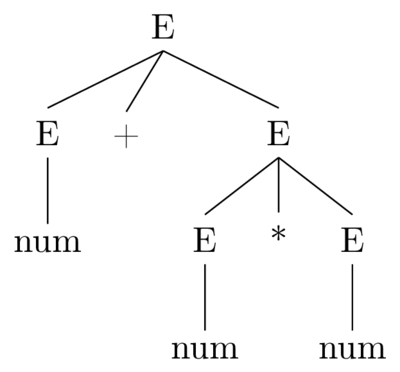
\includegraphics[width=.9\linewidth]{./imgs/image1.png}
\end{center}
\subsection*{Gramáticas livres de contexto}
\label{sec:org15b7711}

\begin{itemize}
\item Em algumas situações é necessário modificar regras de uma gramática para usar certas técnicas de análise sintática.

\item Veremos algumas dessas técnicas.
\end{itemize}
\section*{Transformações de gramáticas}
\label{sec:org0cb1fb3}

\subsection*{Transformações de gramáticas}
\label{sec:org1d6fddf}

\begin{itemize}
\item Fatoração à esquerda: Evitar mais de uma regra com o mesmo prefixo
\end{itemize}
\subsection*{Transformações de gramáticas}
\label{sec:orgcc862d3}

\begin{itemize}
\item Exemplo:
\end{itemize}

\begin{array}{lcl}
  A & \to & xz \,|\, xy\,|\,v
\end{array}

\begin{itemize}
\item pode ser transformada em:
\end{itemize}

\begin{array}{lcl}
  A & \to & xZ\,|\,v\\
  Z & \to & z \,|\,y
\end{array}
\subsection*{Transformações de gramáticas}
\label{sec:org5f9aeca}

\begin{itemize}
\item Introdução de prioridades.
\begin{itemize}
\item Problema comum em linguagens de programação com operadores.
\item Impor ordem de precedência na ausência de parêntesis.
\end{itemize}
\end{itemize}
\subsection*{Transformações de gramáticas}
\label{sec:orgb2e446c}

\begin{itemize}
\item Forma geral para introduzir prioridades:
\begin{itemize}
\item \(E_i\): expressões com precedência de nível \(i\).
\item Maior precedência: mais profundo.
\end{itemize}
\end{itemize}

\begin{array}{lcl}
E_i & \to & E_{i + 1} \,|\, E_i Op_i E_{i + 1}
\end{array}
\subsection*{Transformações de gramáticas}
\label{sec:orgee9d8b6}

\begin{itemize}
\item Eliminar recursão à esquerda
\begin{itemize}
\item Transformar em recursão à direita.
\end{itemize}
\end{itemize}

\begin{array}{lcl}
A & \to & Ay_1\,|\,...\,|\,Ay_n\,|\,w_1\,|\,...\,|\,w_k\\
\end{array}
\subsection*{Transformações de gramáticas}
\label{sec:org9d8485f}

\begin{itemize}
\item Pode ser transformada em
\end{itemize}

\begin{array}{lcl}
A & \to & w_1Z\,|\,...\,|\,w_kZ\,|\,w_1\,...\,|\,w_k\\
Z & \to & y_1Z\,|\,...\,|\,y_nZ\,|\,y_1\,...\,|\,y_n\\
\end{array}
\subsection*{Transformações de gramáticas}
\label{sec:orgbc6e867}

\begin{itemize}
\item Exemplo:
\begin{itemize}
\item \(*\) tem prioridade maior que \(+\)
\end{itemize}
\end{itemize}

\begin{array}{lcl}
E & \to & num \,|\,var\,|\,(E)\,|\,E+E\,|\,E * E\\
\end{array}
\subsection*{Transformações de gramáticas}
\label{sec:org231dd69}

\begin{itemize}
\item Exemplo:
\begin{itemize}
\item \(*\) tem prioridade maior que \(+\)
\end{itemize}
\end{itemize}

\begin{array}{lcl}
E_1 & \to & E_2\,|\,E_1 + E_2\\
E_2 & \to & E_3\,|\,E_2 * E_3\\
E_3 & \to & num\,|\,var\,|\,(E_1)\\
\end{array}
\subsection*{Transformação de gramáticas}
\label{sec:org68724d1}

\begin{itemize}
\item Eliminar recursão a esquerda.
\begin{itemize}
\item Resolução no quadro
\end{itemize}
\end{itemize}

\begin{array}{lcl}
   S & \to & Aa\,|\,b\\
   A & \to & Ac\,|\,Sd\,|\,\lambda\\
\end{array}
\section*{Análise sintática}
\label{sec:orge0d0a8c}

\subsection*{Análise sintática}
\label{sec:orgd510dd7}

\begin{itemize}
\item Dois tipos de algoritmos:
\begin{itemize}
\item Análise sintática top-down
\item Análise sintática bottom-up
\end{itemize}
\end{itemize}
\subsection*{Análise sintática}
\label{sec:org559ec8c}

\begin{itemize}
\item Analisador sintático top-down
\begin{itemize}
\item Inicia a partir do símbolo de partida da gramática.
\item A cada passo, escolhe um não terminal para expandir até
\begin{itemize}
\item Obter o programa de entrada.
\item Encontrar um erro.
\end{itemize}
\end{itemize}
\end{itemize}
\subsection*{Análise sintática}
\label{sec:org110b9dc}

\begin{itemize}
\item Analisador sintático bottom-up
\begin{itemize}
\item Inicia a partir das folhas
\item Encontra substrings da palavra e encontra um lado direito de regra correspondente.
\end{itemize}
\end{itemize}
\subsection*{Análise sintática}
\label{sec:org46cfdd5}

\begin{itemize}
\item Nesta aula, vamos focar em uma técnica top-down.
\begin{itemize}
\item Analisador sintático descendente recursivo.
\end{itemize}
\end{itemize}
\section*{Análise descendente}
\label{sec:orgd902801}

\subsection*{Análise descendente}
\label{sec:orga6e913e}

\begin{itemize}
\item Técnica simples para codificação manual de analisadores sintáticos.

\item Gramáticas são representadas por um conjunto de funções
\begin{itemize}
\item Uma função para cada não terminal.
\end{itemize}
\end{itemize}
\subsection*{Análise descendente}
\label{sec:org7aac418}

\begin{itemize}
\item Analisador para \(A \to X_1 ... X_n\):
\begin{itemize}
\item Para \(i = 1\) até \(n\)
\begin{itemize}
\item Se \(X_i\) for uma variável, chame a função correspondente a \(X_i\).
\item Se \(X_i\) for um terminal, verifique se ele é igual ao primeiro token da entrada.
\end{itemize}
\end{itemize}
\end{itemize}
\subsection*{Análise descendente}
\label{sec:org77d2b75}

\begin{itemize}
\item Vantagem:
\begin{itemize}
\item Codificação simples e de fácil compreensão.
\end{itemize}

\item Problemas:
\begin{itemize}
\item Não permite gramática com recursão à esquerda.
\end{itemize}
\end{itemize}
\subsection*{Análise descendente}
\label{sec:org3910684}

\begin{itemize}
\item Em Haskell, analisadores descendentes são codificados por combinadores.
\end{itemize}
\subsection*{Análise descendente}
\label{sec:orgf7ac51f}

\begin{itemize}
\item Combinadores são uma EDSL para expressar gramáticas.
\begin{itemize}
\item Dúzias de bibliotecas: \texttt{megaparsec}, \texttt{parser-combinators}, \texttt{uu-parselib}, etc\ldots{}
\end{itemize}
\end{itemize}
\subsection*{Análise descendente}
\label{sec:org68852cb}

\begin{itemize}
\item Veremos uma implementação simples de uma EDSL para gramáticas.
\end{itemize}
\subsection*{Análise descendente}
\label{sec:orgbec569e}

\begin{itemize}
\item Representação de parsers
\end{itemize}

\begin{verbatim}
newtype Parser s a =
  Parser { runParser :: [s] -> [(a,[s])] }
\end{verbatim}
\subsection*{Análise descendente}
\label{sec:orge5dd1b0}

\begin{itemize}
\item Parsers são functores
\end{itemize}

\begin{verbatim}
instance Functor (Parser s) where
  fmap f p = Parser (\ s -> [(f x, s') | (x,s') <- runParser p s]) 
\end{verbatim}
\subsection*{Análise descendente}
\label{sec:org890e03b}

\begin{itemize}
\item Parsers são applicatives
\end{itemize}

\begin{verbatim}
instance Applicative (Parser s) where
  pure  a = Parser (\ts -> [(a, ts)])
  p1 <*> p2 = Parser (\ s -> [(f x, s2) | (f, s1) <- runParser p1 s,
                                          (x, s2) <- runParser p2 s1])
\end{verbatim}
\subsection*{Análise descendente}
\label{sec:org051c926}

\begin{itemize}
\item Parsers são alternatives
\end{itemize}

\begin{verbatim}
instance Alternative (Parser t) where
  empty = Parser (\ _ -> [])
  p1 <|> p2 = Parser (\ s -> runParser p1 s ++ runParser p2 s)
\end{verbatim}
\subsection*{Análise descendente}
\label{sec:org96a7130}

\begin{itemize}
\item Parsers são mônadas
\end{itemize}

\begin{verbatim}
instance Monad (Parser t) where
  return =  pure
  p >>= f  = Parser (\ts -> concat [ runParser (f a) cs' |
                                     (a,cs') <- runParser p ts ])
\end{verbatim}
\subsection*{Análise descendente}
\label{sec:orgd386655}

\begin{itemize}
\item Processando o primeiro token da entrada
\end{itemize}

\begin{verbatim}
item :: Parser t t
item = Parser (\ ts ->
                 case ts of
                   []     -> []
                   (c:cs) -> [(c,cs)])
\end{verbatim}
\subsection*{Análise descendente}
\label{sec:org69734de}

\begin{itemize}
\item Processando um token que satisfaz uma condição.
\end{itemize}

\begin{verbatim}
sat :: (t -> Bool) -> Parser t t
sat p = do
          t <- item
          if p t then return t else mzero
\end{verbatim}
\subsection*{Análise descendente}
\label{sec:org0662f66}

\begin{itemize}
\item Processando um certo token.
\end{itemize}

\begin{verbatim}
symbol :: Eq s => s -> Parser s s
symbol c = sat (c ==)
\end{verbatim}
\subsection*{Análise descendente}
\label{sec:org99542fd}

\begin{itemize}
\item Devido a lazy evaluation, podemos entender recursão à esquerda em expressões como uma lista de separadores.

\item Ideia sumarizada pela ER: \(E(op\:E)^*\)
\end{itemize}
\subsection*{Análise descendente}
\label{sec:org48047b8}

\begin{itemize}
\item Função \texttt{chainl}
\end{itemize}

\begin{verbatim}
chainl  ::  Parser s a -> Parser s (a -> a -> a) -> Parser s a
chainl pe po  =  h <$> pe <*> many (j <$> po <*> pe)
  where j op x  =  (`op` x)
        h x fs  =  foldl (flip ($)) x fs
\end{verbatim}
\subsection*{Análise descendente}
\label{sec:org7d2e4f5}

\begin{itemize}
\item Automatizando parsers de expressões
\end{itemize}

\begin{verbatim}
type Op s a = (s, a -> a -> a)

gen :: Eq s => [Op s a] -> Parser s a -> Parser s a
gen ops p = chainl p (choice (map f ops))
  where
    f (s,c) = const c <$> symbol s
\end{verbatim}
\subsection*{Análise descendente}
\label{sec:org1ff8252}

\begin{itemize}
\item Tipo do token
\end{itemize}

\begin{verbatim}
data Token
  = Id String
  | Number Int
  | Add
  | Mult
  | LParen
  | RParen
  deriving (Eq, Show)
\end{verbatim}
\subsection*{Análise descendente}
\label{sec:org127e110}

\begin{itemize}
\item Tipo de expressões
\end{itemize}

\begin{verbatim}
data Expr
  = Var String
  | Lit Int
  | Expr :+: Expr
  | Expr :*: Expr
  deriving (Eq, Show)
\end{verbatim}
\subsection*{Análise descendente}
\label{sec:org262d376}

\begin{itemize}
\item Criando o parser de expressões
\end{itemize}

\begin{verbatim}
exprParser :: Parser Token Expr
exprParser = addtable `gen` termParser
  where
    addtable = [(Add, (:+:))]
\end{verbatim}
\subsection*{Análise descendente}
\label{sec:org0915dfa}

\begin{itemize}
\item Parser para termos
\end{itemize}

\begin{verbatim}
termParser :: Parser Token Expr
termParser = multable `gen` factParser
  where
    multable = [(Mult, (:*:))]
\end{verbatim}
\subsection*{Análise descendente}
\label{sec:org3112ef0}

\begin{itemize}
\item Parser para fatores
\end{itemize}

\begin{verbatim}
factParser :: Parser Token Expr
factParser = numParser  <|>
             varParser  <|>
             parenExpr
  where
    parenExpr = pack lparen exprParser rparen
    lparen = symbol LParen
    rparen = symbol RParen
\end{verbatim}
\section*{Concluindo}
\label{sec:org89b8f78}

\subsection*{Concluindo}
\label{sec:org5692da5}

\begin{itemize}
\item Apresentamos uma introdução à análise sintática.

\item Revisamos sobre GLCs e transformações sobre estas.
\end{itemize}
\subsection*{Concluindo}
\label{sec:org679a980}

\begin{itemize}
\item Apresentamos a técnica de análise sintática descendente recursiva.

\item Em Haskell, esta técnica é representada por combinadores.
\end{itemize}
\subsection*{Concluindo}
\label{sec:orgd3a52ec}

\begin{itemize}
\item Próxima aula: análise sintática LL(1).
\end{itemize}
\section*{Exercícios}
\label{sec:org1da737a}

\subsection*{Exercícios}
\label{sec:org4f4a5ec}

\begin{itemize}
\item Construa um analisador sintático descendente recursivo para seguinte
linguagem de fórmulas da lógica proposicional.
\end{itemize}

\begin{array}{lcl}
F & \to & \textbf{true}\,|\,\textbf{false}\,|\,\textbf{not }\,F\,|\,F\:\:\textbf{/\\}\:\:F\,|\,F\:\:\textbf{\\/}\:\:F\\
\end{array}
\end{document}
